\documentclass[11pt]{book}
\usepackage{muromm}
\usepackage[inline]{asymptote}

\usepackage[Sonny]{fncychap} % fancy chapters
\ChTitleVar{\huge}

\usepackage[tocflat]{tocstyle} % TOC generation
\usetocstyle{standard}

\usepackage{titlesec} % section customization


\titleformat{\section}[block]{\Large\bfseries}{\thesection.}{0.5em}{}

\pagestyle{fancy}
%\lfoot{\sffamily\bfseries\hyperlink{tabla}{Índice}}

%HyperSETUP
\hypersetup{
    colorlinks= true,
    urlcolor= cyan,
    linkcolor= purpleLinks,
    citecolor=red,
    pdftitle={muromm},
    bookmarks = true,
    pdfpagemode = FullScreen,
}

\begin{document}

\title{Manifiesto Universal de Recursos para la Olimpiada Mexicana de Matemáticas}
\author{Diego Caballero Ricaurte, Proyecto MURO}
\date{2023}

\maketitle
\null\vfill
\begin{center}
    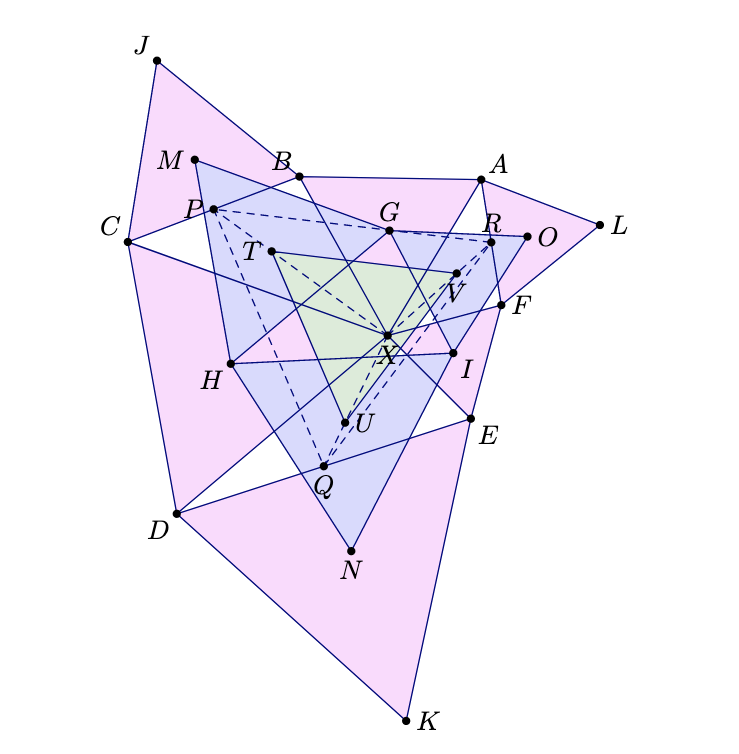
\includegraphics{images/muro.png}
\end{center}
\null\vfill

\hypertarget{tabla}{\tableofcontents}

% Introducción

\chapter{Introducción}

    \section{ProyectoMURO}

    \section{¿Qué es MUROMM?}

    \section{Conceptos Básicos}

% Álgebra

\chapter{Álgebra}

    \section{Manipulación Algebráica}

    \section{Polinomios}

    \section{Ecuaciones Funcionales}

    \section{Desigualdades}

% Combinatoria

\chapter{Combinatoria}

    \section{Conteo}

    \section{Invarianza}

    \section{Teoría de Juegos}

    \section{Gráficas}

    \section{Geo-Combi}


% Geometría

\chapter{Geometría}

    \section{Ángulos y Líneas}

    \section{Triángulos I}

    \section{Cuadriláteros Cíclicos}

    \section{Cómo resolver problemas de Geometría}

    \section{Triángulos II}

    \section{Geometría Proyectiva}


% Teoría de Números

\chapter{Teoría de Números}

    \section{Módulos, Divisibilidad, y Primos}

    \section{Exponentes}

    \section{Otros Teoremas}


% Misceláneo

\chapter{Misceláneo}

    \section{Sugerencias para exámenes}

    \section{Entrenamiento}

% Problemas

\chapter{Problemas}

    \section{Problemas OMM}

    \section{Problemas por nivel}

% Soluciones

\chapter{Soluciones}

    \section{Soluciones OMM}

    \section{Soluciones por nivel}

% Apéndice

\chapter{Apéndice}

    \section{Índice}

    \section{Definiciones y Notación}

    \section{Colaboradores y Agradecimientos}

    \section{Bibliografía}

\end{document}